% System architecture and event flow (build: pdflatex system-architecture.tex -> system-architecture.pdf)
\documentclass[tikz,border=4pt,11pt]{standalone}
\usepackage[T1]{fontenc}
\usepackage{lmodern}
\usetikzlibrary{shapes.geometric,positioning,fit,arrows.meta,backgrounds}
\begin{document}
\sffamily
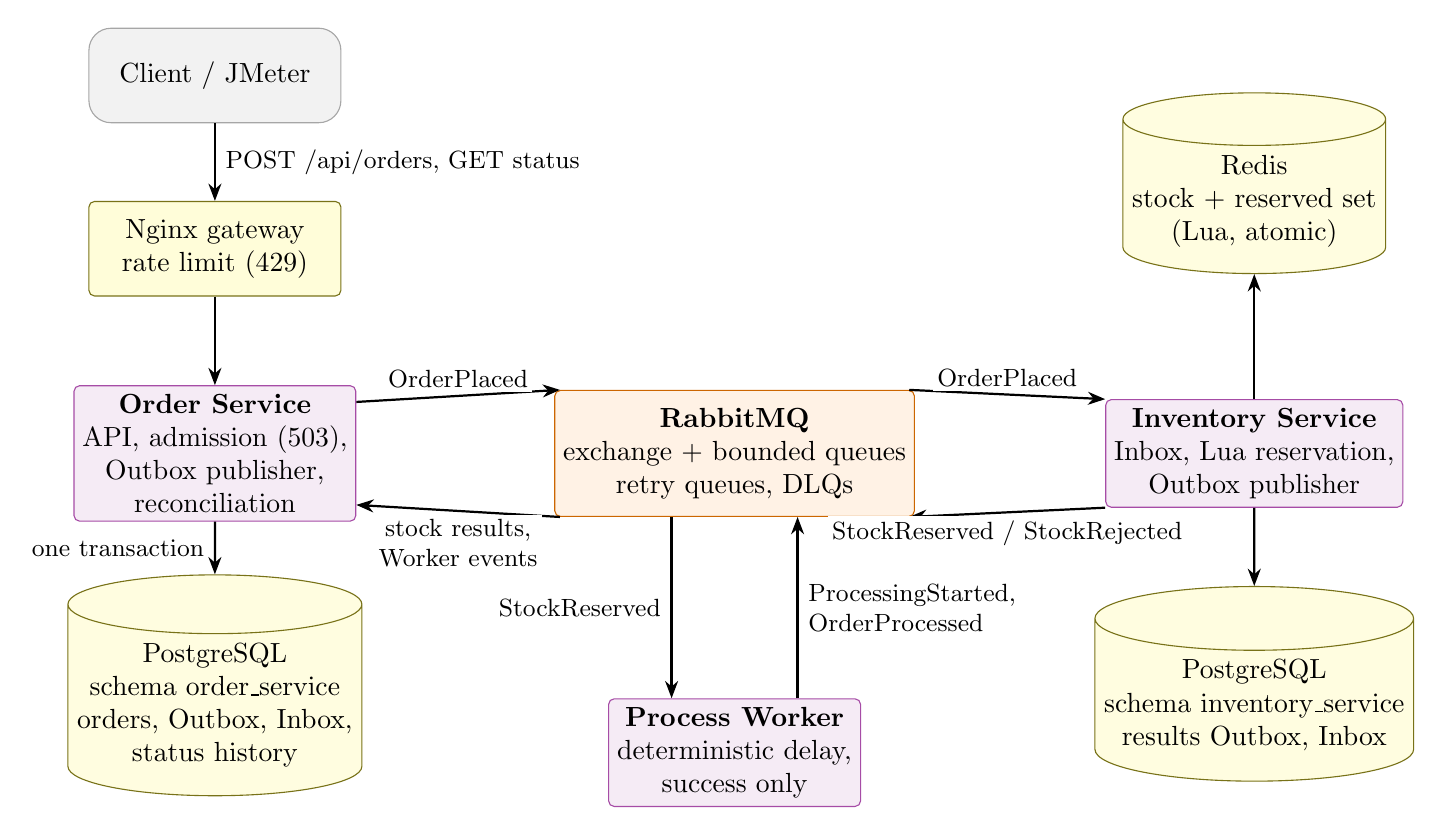
\begin{tikzpicture}[
  >={Stealth[length=2.2mm]},
  svc/.style={draw=violet!70, fill=violet!8, rounded corners=2pt, align=center,
              minimum height=12mm, minimum width=32mm, inner sep=3pt},
  ext/.style={svc, draw=gray!70, fill=gray!10, rounded corners=8pt},
  db/.style={cylinder, shape border rotate=90, aspect=0.2, draw=olive!80!black,
             fill=yellow!12, align=center, minimum width=30mm, minimum height=13mm},
  mq/.style={svc, draw=orange!80!black, fill=orange!10},
  flow/.style={->, thick},
  ev/.style={font=\small, fill=white, inner sep=1.5pt}
]
\node[ext] (client) at (0,0) {Client / JMeter};
\node[svc, draw=olive!80!black, fill=yellow!15] (nginx) at (0,-2.2) {Nginx gateway\\rate limit (429)};
\node[svc] (order) at (0,-4.8) {\textbf{Order Service}\\API, admission (503),\\Outbox publisher,\\reconciliation};
\node[db] (pgo) at (0,-8.0) {PostgreSQL\\schema order\_service\\orders, Outbox, Inbox,\\status history};
\node[mq, minimum width=40mm, minimum height=16mm] (mq) at (6.6,-4.8) {\textbf{RabbitMQ}\\exchange + bounded queues\\retry queues, DLQs};
\node[svc] (inv) at (13.2,-4.8) {\textbf{Inventory Service}\\Inbox, Lua reservation,\\Outbox publisher};
\node[db] (redis) at (13.2,-1.6) {Redis\\stock + reserved set\\(Lua, atomic)};
\node[db] (pgi) at (13.2,-8.0) {PostgreSQL\\schema inventory\_service\\results Outbox, Inbox};
\node[svc] (worker) at (6.6,-8.6) {\textbf{Process Worker}\\deterministic delay,\\success only};

\draw[flow] (client) -- node[ev, right=2pt] {POST /api/orders, GET status} (nginx);
\draw[flow] (nginx) -- (order);
\draw[flow] (order) -- node[ev, left=2pt] {one transaction} (pgo);
\draw[flow] (order.20) -- node[ev, above=1pt] {OrderPlaced} (mq.160);
\draw[flow] (mq.20) -- node[ev, above=1pt] {OrderPlaced} (inv.160);
\draw[flow] (inv.200) -- node[ev, below=1pt] {StockReserved / StockRejected} (mq.340);
\draw[flow] (mq.200) -- node[ev, below=1pt, align=center] {stock results,\\Worker events} (order.340);
\draw[flow] (inv) -- (redis);
\draw[flow] (inv) -- (pgi);
\draw[flow] ([xshift=-8mm]mq.south) -- node[ev, left=2pt] {StockReserved} ([xshift=-8mm]worker.north);
\draw[flow] ([xshift=8mm]worker.north) -- node[ev, right=2pt, align=left] {ProcessingStarted,\\OrderProcessed} ([xshift=8mm]mq.south);
\end{tikzpicture}
\end{document}
